\documentclass[12pt,letterpaper]{article}
\usepackage[utf8]{inputenc}
\usepackage[spanish, es-tabla]{babel}
\usepackage[version=3]{mhchem}
\usepackage[journal=jacs]{chemstyle}
\usepackage{amsmath}
\usepackage{amsfonts}
\usepackage{amssymb}
\usepackage{makeidx}
\usepackage{graphicx}
\usepackage{xcolor}
\usepackage[stable]{footmisc}
\usepackage[section]{placeins}
%Paquetes necesarios para tablas
\usepackage{longtable}
\usepackage{array}
\usepackage{xtab}
\usepackage{floatrow}
\usepackage{multirow}
\usepackage{colortab}
\usepackage{caption}
\usepackage{enumitem}
%Paquete para el manejo de las unidades
\usepackage{siunitx}
\sisetup{mode=text, output-decimal-marker = {,}, per-mode = symbol, qualifier-mode = phrase, qualifier-phrase = { de }, list-units = brackets, range-units = brackets, range-phrase = --}
\usepackage{cancel}
%Paquetes necesarios para imágenes, pies de página, etc.

\usepackage{listings}
\usepackage{color}

\definecolor{dkgreen}{rgb}{0,0.6,0}
\definecolor{gray}{rgb}{0.5,0.5,0.5}
\definecolor{mauve}{rgb}{0.58,0,0.82}

\lstset{frame=tb,
  language=Java,
  aboveskip=3mm,
  belowskip=3mm,
  showstringspaces=false,
  columns=flexible,
  basicstyle={\small\ttfamily},
  numbers=none,
  numberstyle=\tiny\color{gray},
  keywordstyle=\color{blue},
  commentstyle=\color{dkgreen},
  stringstyle=\color{mauve},
  breaklines=true,
  breakatwhitespace=true,
  tabsize=3
}

%Instrucción para evitar la indentación
%\setlength\parindent{0pt}
%Paquete para incluir la bibliografía
\usepackage[backend=bibtex,style=chem-acs,biblabel=dot]{biblatex}
\addbibresource{references.bib}


%Modificación del formato de los captions
\usepackage[margin=10pt,labelfont=bf]{caption}

%Paquete para incluir comentarios
\usepackage{todonotes}

%Paquete para incluir hipervínculos
\usepackage[colorlinks=true, 
            linkcolor = blue,
            urlcolor  = blue,
            citecolor = black,
            anchorcolor = blue]{hyperref}

\begin{document}
\renewcommand{\labelitemi}{$\checkmark$}

\renewcommand{\CancelColor}{\color{red}}

\newcolumntype{L}[1]{>{\raggedright\let\newline\\\arraybackslash}m{#1}}

\newcolumntype{C}[1]{>{\centering\let\newline\\\arraybackslash}m{#1}}

\newcolumntype{R}[1]{>{\raggedleft\let\newline\\\arraybackslash}m{#1}}


\begin{center}

	\textbf{SIMULACION DE MODELOS POBLACIONALES}\\
	\vspace{7mm}
	\textbf{\large{Realizado Por: Michael Santiago Díaz 160002613}}\\
	\textbf{\large{Entregado A: Ph.D Ángel Cruz}}\\
	\vspace{5mm}
	\textbf{\large{Universidad de los llanos}}\\
	\today
\end{center}

\section{Introduction}

Este informe de simulación comprende el modelo de población de cierto rango de características que describe un texto, que paso a paso se va tornando un poco más complejo debido a las formas descriptivas de trabajo que se requiere para entender el modelo de simulación poblacional.

\section{Analisis  de Datos}
\label{sec:examples}

\subsection{Ejemplo 1}
Se crea un modelo con un nivel llamado población y un flujo de entrada (Nacimientos), después de hacer el proceso se puede observar y analizar que nacen 150 personas por año el proceso es constante cada año y la población cada año se va incrementando.
\begin{figure}
\centering
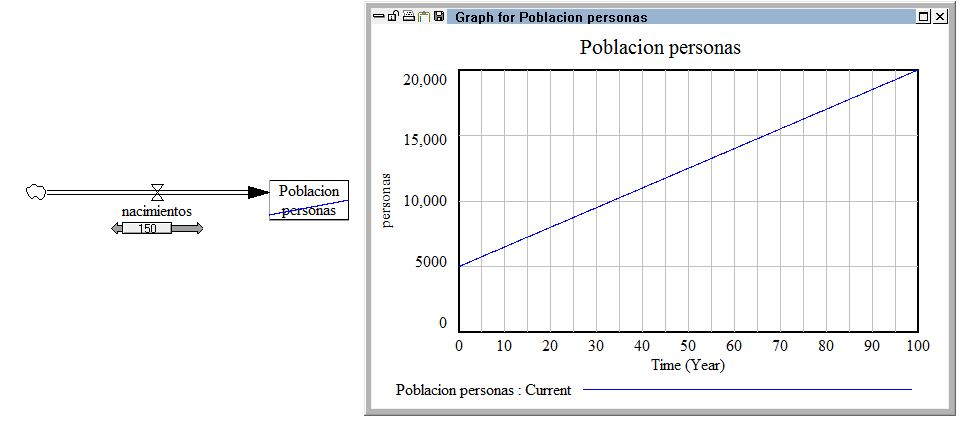
\includegraphics[width=10cm, height=5cm]{1.JPG}
\end{figure}

\subsection{	Ejemplo 2}

En este segundo ejemplo se construyó un segundo flujo pero este es de salida (muertes), y se analizó en la gráfica que las muertes es proporcional a los nacimientos, ósea que entre más personas nazcan más personas irán muriendo.

\begin{figure}
\centering
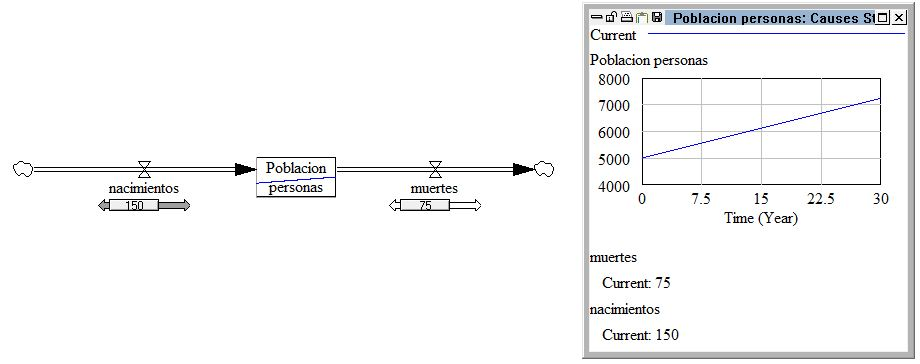
\includegraphics[width=10cm, height=5cm]{2.JPG}
\end{figure}

\subsection{Ejemplo 3}
En este tercer ejemplo se cambiaron los valores de entrada (nacimientos) y salida (muertes), se observa que van decreciendo las personas al pasar de los años, pues la cantidad de muertes cada año son más que la cantidad de nacimientos.
\begin{figure}
\centering
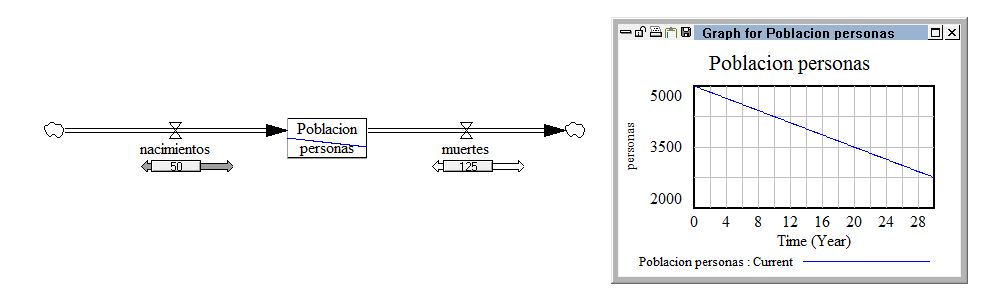
\includegraphics[width=10cm, height=5cm]{3.JPG}
\end{figure}

\section{Feedback}
En este paso se continuo agregando dos variables al sistema fracción de nacimientos y fracción de muertes, la fracción de nacimientos se calculó dividiendo la tasa de nacimientos entre el total de la población existente (150/5000=0,03), y la fracción de muertes igualmente se dividió la tasa de mortalidad entre la cantidad de población.
Se puede concluir que entre más población mas nacimientos y entre más población mayor es la fracción muertes.
Ya que fueron dos casos diferentes, en estas imágenes se ven reflejados los procesos simulados.

\begin{figure}
\centering
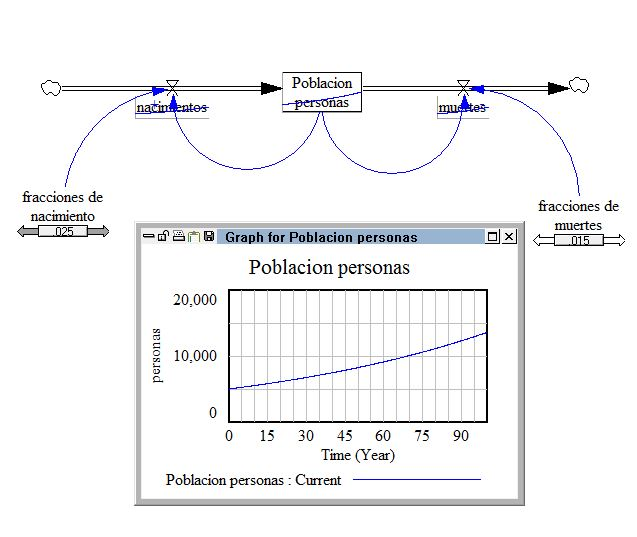
\includegraphics[width=10cm, height=5cm]{4.JPG}
\end{figure}
\begin{figure}
\centering
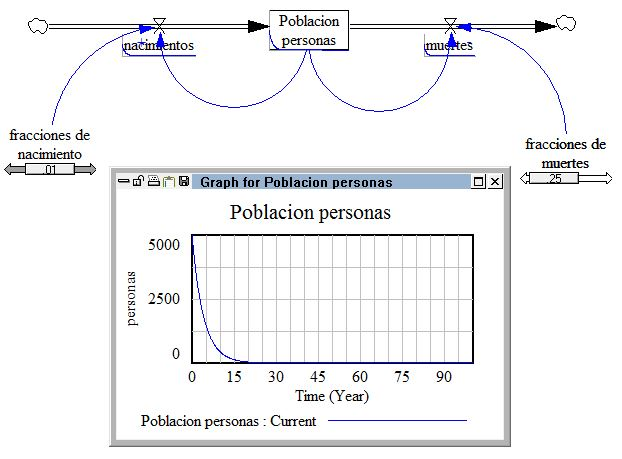
\includegraphics[width=10cm, height=5cm]{5.JPG}
\end{figure}
\section{Modelo logístico }

Este es un crecimiento exponencial en forma de S, conocido como crecimiento logístico, se caracteriza cuando la retroalimentación genera un crecimiento exponencial, este es compensado por la retroalimentación negativa que obliga a cierta población a estabilizarse.

\subsection{Estructura genérica }
 
Estos tipos de modelos que acompañan este estilo logístico se caracterizan por un crecimiento acotado, se explica el ejemplo de los conejos:
\begin{itemize}
\item Cierta población de conejos viven en un bosque con recursos limitados, como se sabe entre más conejos existan más elevada será la tasa de nacimientos, ósea que el número de conejos que comen pasto aumentara, esto también trae consecuencias como se habló de recursos limitados, digamos que el agua es limitada o acotada para cierta cantidad de conejos, muchos conejos se van a quedar sin agua o no tomaran lo suficiente para poder subsistir  y luego estos conejos mueren hasta que con el tiempo alcance de nuevo el agua para la cantidad de conejos actuales, con este suceso se tiende a haber una estabilidad en el sistema.   
\end{itemize}

\begin{figure}
\centering
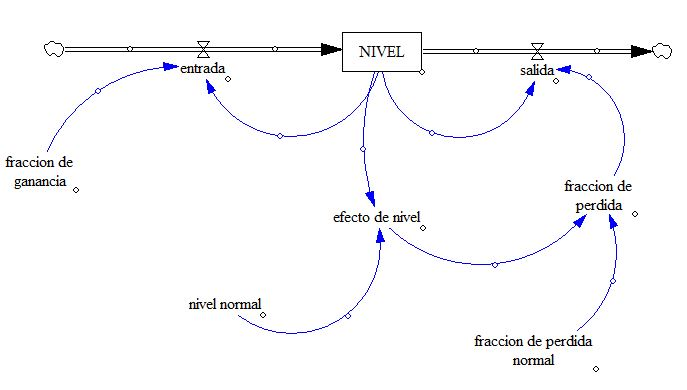
\includegraphics[width=10cm, height=5cm]{6.JPG}
\caption{\label{fig: } Modelo de recursos limitados }
\end{figure}

\subsection{Modelo para estudiar el crecimiento de una población de conejos}

En este paso se representó en diagrama que analiza el crecimiento de la población de conejos que se habló anterior mente que contaba con recursos limitados.

\begin{figure}
\centering
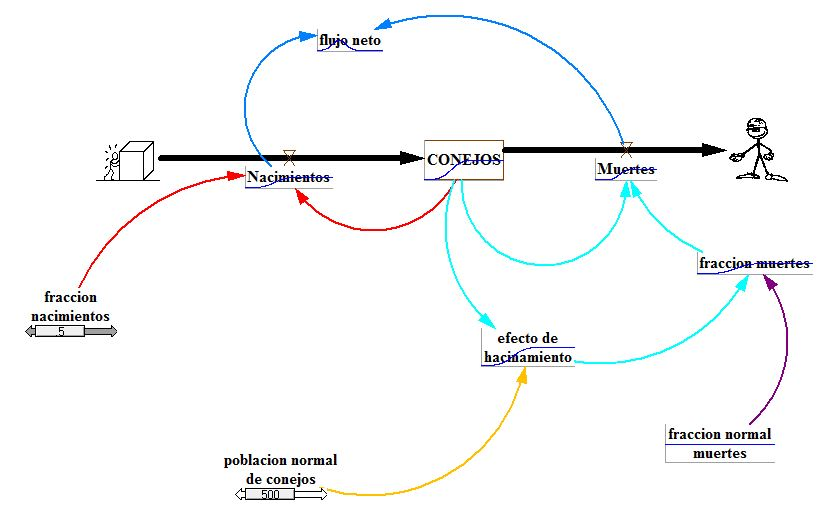
\includegraphics[width=10cm, height=5cm]{7.JPG}
\caption{\label{fig: } Grafica diagrama con problema propuesto  }
\end{figure}

La siguiente es la grafica que muestra el crecimiento gradua y que tiende a una constante o mas conocido como crecimiento en forma de S.

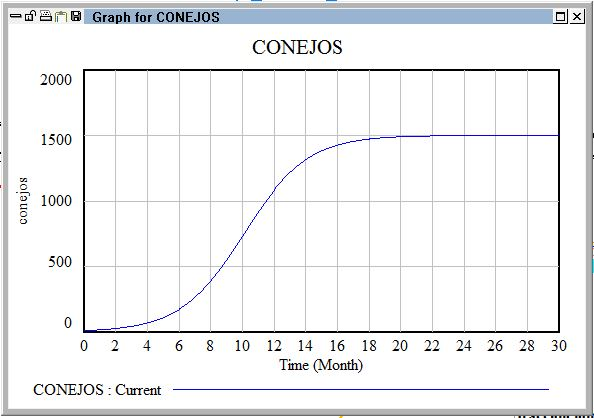
\includegraphics[width=10cm, height=5cm]{8.JPG}

\begin{figure}
\centering
\caption{\label{fig: } Modelo de problema propuesto  }
\end{figure}

\section{Conclusiones}
	Vensim es un programa que nos permite simular casos sencillos de manera rapida y tambien permite una rapida modificació de los modelos para adaptarlos a ciertas situaciones.


\end{document}